\chapter{Introducción específica} % Main chapter title

\label{Chapter2}

En este capítulo se describe el contexto y el protocolo bajo los que se espera que el modelo funcione. También se describen los conceptos de inteligencia artificial aplicados y las consideraciones físicas que se tuvieron en cuenta. Además se mencionan las herramientas de software utilizadas.

\section{Protocolo}

Cuando un centro de salud adquiere o alquila un equipo se los capacita para su uso correcto. En la capacitación se menciona un protocolo que es recomendable utilizar para el desarrollo del tratamiento. Esto nace del estudio de los tratamientos en general y de las particularidades del equipo.
El sistema permite regular la temperatura de un paciente neonatal a partir de establecer un objetivo. Esto ofrece una gran variedad de campos de uso, pero el principal caso es el de utilizar el equipo para inducir hipotermia. Por esto, se establece el protocolo para este caso como se describe a continuación:

\begin{itemize}
	\item Se debe colocar al paciente dentro de una incubadora.
	\item El paciente debe estar sedado.
	\item La temperatura objetivo debe ser de 33,5 ºC.
	\item No se debe mover al niño.
\end{itemize}

Bajo estas condiciones el funcionamiento del equipo es muy bueno, el error en las mediciones se reduce y se mantiene al paciente en una temperatura estable. En la imagen \ref{fig:recorte-equipo} se puede ver como evoluciona la temperatura del paciente, tomado de la pantalla del equipo. 

\begin{figure}[h]
	\centering
	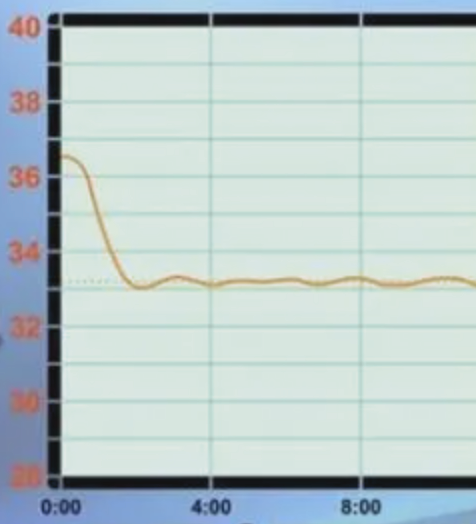
\includegraphics[width=0.6\textwidth]{./Figures/recorte-equipo.png}
	\caption{Evolución de la temperatura del paciente.}
	\label{fig:recorte-equipo}
\end{figure}

\newpage
\section{Contextos de uso del equipo}

Si bien se detalla el protocolo a seguir, y en muchos casos se tiene en cuenta, existen casos en los que no. En algunos tratamientos la temperatura objetivo es establecida en 32.5 ºC, y en otros fue establecida en otros valores, entre los 30 ºC y los 35 ºC. Además se dan situaciones en las que el paciente no está correctamente sedado en la incubadora. Esto produce que el equipo tarde más de lo usual en llevarlo al objetivo y que la oscilación de la temperatura del paciente sea mayor. También se da que se mueve al niño, y esto produce que en ese momento la temperatura diste del objetivo. Estos contextos se comparan en la tabla \ref{tab:contextos-uso}. 

\begin{table}[h]
	\centering
	\caption[Contextos de uso]{Comparación de contextos de uso.}
	\begin{tabular}{l c}  
		\toprule
		\textbf{Situación} 	 & \textbf{Consecuencia}  \\
		\midrule
		Temperatura objetivo distinta & Tratamiento no estándar e impreciso \\		
		Paciente que no está sedado  & Tratamiento impreciso  \\
		Se mueve al paciente & Tratamiento impreciso por un lapso de tiempo \\		
		\bottomrule
		\hline
	\end{tabular}
	\label{tab:contextos-uso}
\end{table}

Como se mencionó, estos contextos de uso reducen la eficiencia del funcionamiento del equipo. Esto genera una oportunidad para el nuevo modelo. Se espera que esta nueva herramienta tenga mayor robustez y se comporte mejor ante contextos diversos. Esto puede lograrse a partir de un aprendizaje sólido y de un conjunto de datos amplio. Además diversas estrategias pueden ser aplicadas para maximizar la robustez del modelo. Esto se comentará en el siguiente capítulo.

\section{Redes neuronales informadas por física}
En esta sección se describen conceptos generales de redes neuronales y el enfoque de redes informadas por física, que son los fundamentos el desarrollo de los modelos.

\newenvironment{conditions}
{\par\vspace{\abovedisplayskip}\noindent\begin{tabular}{>{$}l<{$} @{${}={}$} l}}
	{\end{tabular}\par\vspace{\belowdisplayskip}}

\subsection{Redes neuronales}
Para el desarrollo de este trabajo se utilizaron diversos algoritmos de inteligencia artificial, siendo las redes neuronales las que mejores resultados presentaron. 
Las redes neuronales artificiales (RNA) son modelos computacionales que se inspiran en el funcionamiento del cerebro humano. La unidad de procesamiento fundamental de las redes neuronales suele ser denominada perceptrón o neurona.  Este recibe un vector de señales de entrada $ x =(x_1, x_2, . . . , x_n) $, las cuales se multiplican por un vector de pesos $W = (w_1, w_2, . . . , w_n)$. Esto se resume en la siguiente suma $\sum_{i=1}^n x_i  w_i$
También se añade valor denominado sesgo, que es un término independiente cuyo fin es otorgar flexibilidad en el aprendizaje de conceptos.
Por último a la salida de cada perceptrón se le aplica una transformación no lineal, llamada función de activación $g(z)$.  En conclusión, la salida de cada neurona se expresa como \ref{eq:neurona}.

\begin{equation}
	\label{eq:neurona}
	\hat{y} = g(z) = \sum_{i=1}^n x_i  w_i + b
\end{equation}

Para este modelo la función de activación que mejores resultados otorgó es la tangente hiperbólica, definida como $tanh(x) = \frac{e^x - e^{-x}}{e^x + e^{-x}} = \frac{1 - e^{-2x}}{1 + e^{-2x}}$.

En particular en este trabajo se desarrollaron modelos de aprendizaje profundo, que son redes neuronales multicapa \citep{Goodfellow-et-al-2016}. Estas arquitecturas están compuestas por al menos 3 capas. La primera es denominada capa de entrada, que suele tener tantas neuronas como la longitud de los vectores de entrada. A ésta le sigue la capa oculta, y luego sigue una capa de salida, con tantas neuronas como la longitud del vector de salida del modelo.

El aprendizaje en estos modelos se da a partir de una función de entrenamiento cuyo objetivo es minimizar el error en las predicciones. Definida una función de error $L(\hat{y},y)$, el objetivo es minimizar su valor. En este caso se utilizó el entrenamiento por descenso del gradiente. En este algoritmo el error se reduce de forma iterativa buscando un mínimo en la función a través del gradiente. En cada iteración se calcula el siguiente punto en el espacio como una resta entre el punto actual y el gradiente en ese punto multiplicado por un factor de aprendizaje. Desde el punto de vista geométrico, al restar el gradiente lo que sucede es que se están modificando los pesos hacia la dirección donde crece la función, esto es, hacia algún mínimo, que puede ser local o global. Este proceso se repite hasta alcanzar un número máximo de iteraciones. En términos generales ésto se puede representar con la ecuación $p_{i+1} = p{i} - \gamma \nabla L(\hat{y},y)$. Esto se propaga para modificar los pesos de cada neurona mediante la técnica de \textit{back propagation } \citep{Goodfellow-et-al-2016}.

Este comportamiento se describe en la figura \ref{fig:gradient}. Se visualiza que para un punto $T_i$ se calcula al punto $T_{i+1}$ en la dirección geométrica del mínimo local.

\begin{figure}[htbp]
	\centering
	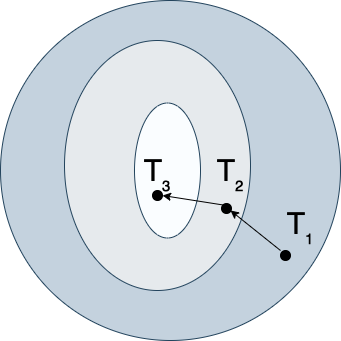
\includegraphics[width=0.5\textwidth]{./Figures/gradient.png}
	\caption{Ilustración del algoritmo de descenso del gradiente.}
	\label{fig:gradient}
\end{figure}

\subsection{Consideraciones físicas}
En principio, existe una temperatura mínima y máxima para el agua que circula en el equipo. El rango válido es entre 5 ºC y 40 ºC. Sin embargo en la práctica no es normal que el agua circule a temperaturas menores a 15 ºC por lo que podemos considerar como primer limitación física que la temperatura del agua esté entre los 15 ºC y los 40 ºC.  Por esto la misma respeta la expresión \ref{eq:umbrales_temperatura}.

\begin{equation}
	\label{eq:umbrales_temperatura}
	t : t >= 15 \circ \land  t <= 40 \circ
\end{equation}

Otra consideración es que se deben evitar en lo posible los cambios bruscos de temperatura. El algoritmo actual intenta generar cambios de 0,1 ºC. Si bien esto no es un requerimiento, las buenas prácticas en este tipo de tratamientos indican que la temperatura no cambie de forma brusca. Entonces, la bondad del modelo es inversamente proporcional a la magnitud del cambio de temperatura. Esto queda expresado en \ref{eq:bondad_vs_cambio_t}.

\begin{equation}
	\label{eq:bondad_vs_cambio_t}
	Bondad\propto \frac{1}{T_i - T_{i+1}}
\end{equation}

Dado que la respuesta del modelo es una temperatura a la que se debe calentar o enfriar el agua, se tiene en cuenta la energía necesaria para el cambio de temperatura a aplicar. Para esto se plantea en la ecuación \ref{eq:e_cambio_t} la energía requerida.

\begin{equation}
	\label{eq:e_cambio_t}
	E = m c \Delta T
\end{equation}

donde
\begin{conditions}
	m     &  masa del agua \\
	c     &  capacidad calorífica del agua \\   
	T &  temperatura
\end{conditions}

En términos generales, los modelos de inteligencia artificial vistos funcionan como sistemas de caja negra \citep{ML_methods}, es decir, modelos cuyo funcionamiento resulta muy difícil de explicar. Dadas las condiciones físicas del problema, se prefirió un enfoque de caja gris \citep{YANG2024121523}, que busca tener mayor control en su funcionamiento y por esto, una mejor capacidad para entender su comportamiento.
Para lograr esto se buscó incorporar las condiciones mencionadas al modelo. Se utilizó el enfoque de redes informadas por física \citep{cuomo2022scientificmachinelearningphysicsinformed}. Este tipo de redes se diseñó como una solución para los modelos de aprendizaje profundo diseñados para resolver problemas gobernados por principios físicos esenciales. En este paradigma se restringen las predicciones a soluciones coherentes con tales principios. Para esto incorporan en su aprendizaje los modelos físicos que gobiernan al problema. Esto proporciona una gran versatilidad ya que se tiene la capacidad de aprender de los datos y la de mantener las ecuaciones físicas que rigen en el problema. Para lograr esto, en este trabajo se definió una función de costo específica. Esta función tiene en consideración las ecuaciones vistas en esta sección y la función de error original, que es la diferencia entre la temperatura generada en el paciente y la objetivo. En el siguiente capítulo se explica como se diseñó esta solución.

En la figura \ref{fig:loss} se muestra un ejemplo de una función de error. El algoritmo de entrenamiento puede converger en algún mínimo local. Para este ejemplo, el mínimo de la sección mas clara de la gráfica es un mínimo que no cumple con las condiciones físicas. Siguiendo esta función para el entrenamiento, es posible que el modelo converja a la solución que no cumple las propiedades físicas del problema. 

\begin{figure}[htbp]
	\centering
	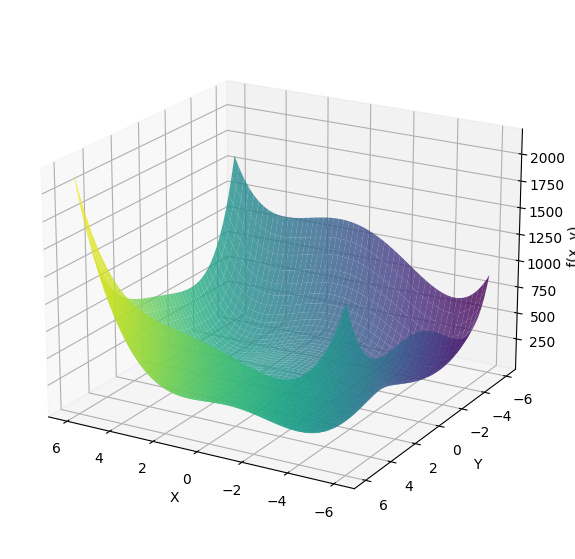
\includegraphics[width=0.6\textwidth]{./Figures/loss_example.png}
	\caption{Ejemplo de función de costo.}
	\label{fig:loss}
\end{figure}

Mediante redes informadas por física se puede modificar la función de costo, penalizando estas secciones, dejando como mínimos a los que cumplan con las propiedades. En la figura \ref{fig:modified-loss} se muestra un ejemplo como puede quedar la función de costo luego de incorporar los conceptos físicos.

\begin{figure}[htbp]
	\centering
	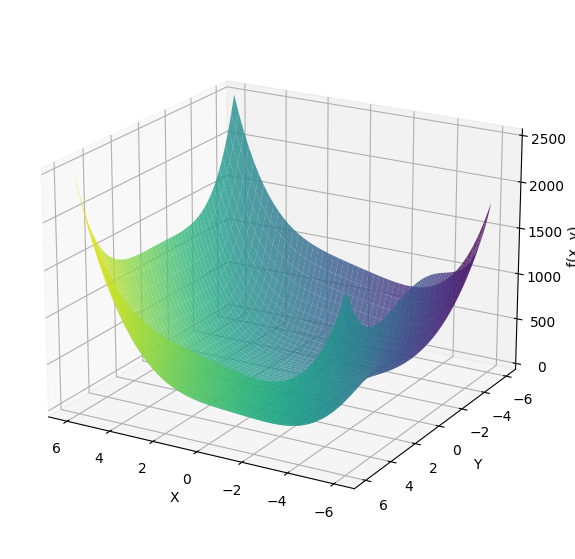
\includegraphics[width=0.6\textwidth]{./Figures/costo-modificada.png}
	\caption{Ejemplo de función de costo.}
	\label{fig:modified-loss}
\end{figure}

\section{Herramientas de software}
Como lenguaje de programación se utilizó Python \citep{python}. Este es un lenguaje de programación de alto nivel, interpretado, y multiparadigma. Cuenta con numerosas funciones propias del lenguaje que facilitan el desarrollo, y una amplia comunidad de soporte. Además es un lenguaje estándar en soluciones de inteligencia artificial.
También se utilizó Jupyter-Notebook \citep{jupyter}, que es un proyecto que facilita la programación interactiva. Permite dividir al código en celdas y ejecutar todas las sentencias que estén contenidas en una celda. 
Para el desarrollo de este trabajo se utilizó Visual Studio como entorno de desarrollo integrado. Este entorno permite desarrollar y ejecutar de forma amigable tanto archivos puros en Python como otros con extensión .ipynb, que son los que siguen el proyecto Jupyter-Notebook y el paradigma de ejecución por celdas. Esto permitió un desarrollo ágil de los modelos y los módulos necesarios.

Este trabajo se basó en herramientas de software útiles y de calidad comprobada en la industria por ser estándares. Para la manipulación de diversos objetos matemáticos se utilizó Numpy \citep{numpy}, que es una biblioteca potente que ofrece múltiples facilidades para éstas prácticas. 
Mediante Matplotlib \citep{matplotlib} se visualizaron gráficos que permiten entender mejor las relaciones entre los datos y las comparaciones realizadas. 
TensorFlow \citep{tensorflow} en general y Keras \citep{keras} en particular como frameworks para construir redes neuronales, debido a su potencia y a su flexibilidad para definir una función de costo específica y confiable.
Además se utilizó Scikit-Learn \citep{scikit-learn} como framework para implementar modelos de inteligencia artificial auxiliares y la realización de pruebas preliminares, como para segmentar datos y calcular meta datos.

En la figura \ref{fig:software} se muestra un diagrama que busca explicar las herramientas utilizadas y su relación. En el centro están los frameworks de desarrollo de modelos de inteligencia artificial, que son atravesados por herramientas trasversales como Numpy y Matplolib, y están contenidos en Python que es el lenguaje de programación utilizado.

\begin{figure}[htbp]
	\centering
	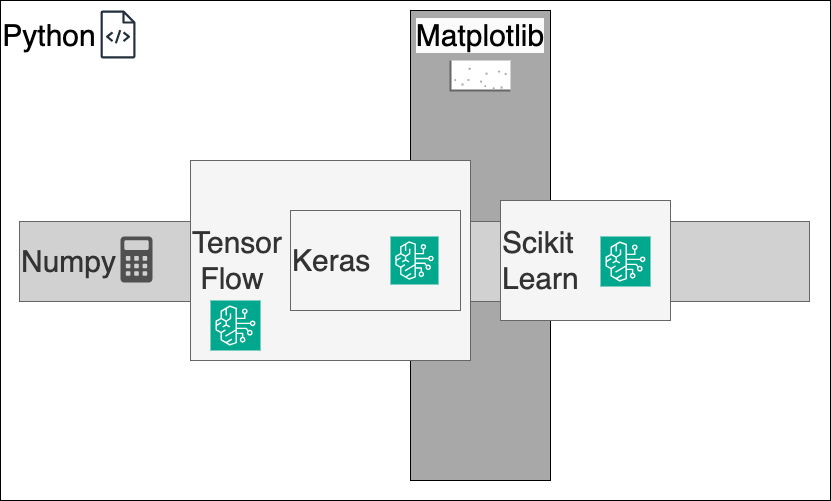
\includegraphics[width=1\textwidth]{./Figures/software.png}
	\caption{Diagrama de herramientas de software.}
	\label{fig:software}
\end{figure}
